\section{Proximate Programming Interface and API} \label{sec:prog}

This section gives an overview of Proximate programming interface or API
and how one would program the entire application using proximate API.
And then we will describe the task based queuing model we have implemented
for proximate to scheduled tasks for in-order cores as well as Softbrain.

\subsection{Proximate API}
At a high-level Proximate API is very much similar to any task based
API like Cilk~\cite{leiserson2010cilk++} or TBB~\cite{pheatt2008intel}.
The only difference is the way memory gets allocated in each of the
vault and the data sharding part where the programmer has to explicitly do a 
copy of the data structures to each of these vault allocated structures. 

\paragraph{Kernel Context and Loading}

\begin{figure}[h]
  \begin{center}
    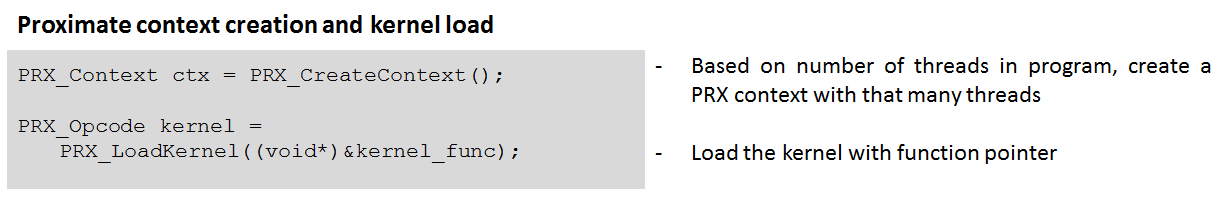
\includegraphics[width=\linewidth]{cs758-figs/api-alloc.png}
  \end{center}
\vspace{-0.2in}
  \caption{API for Context Creation and Kernel Loading}
  \label{fig:api-kernel}
\vspace{-0.05in}
\end{figure}

Figure~\ref{fig:api-kernel} shows the code snippet for Kernel creation
and loading the kernel to device memory location. 
This API can be used by the programmer to register a function/kernel, 
located in the host address space, with the Proximate library. 
The input argument is the function pointer to the kernel in the host virtual address space.
The return value is the index of the page in the Proximate “code Region”.   

\paragraph{Memory Allocation}
The next API is for the memory management on Proximate memory mapped region. 

\begin{figure}[h]
  \begin{center}
    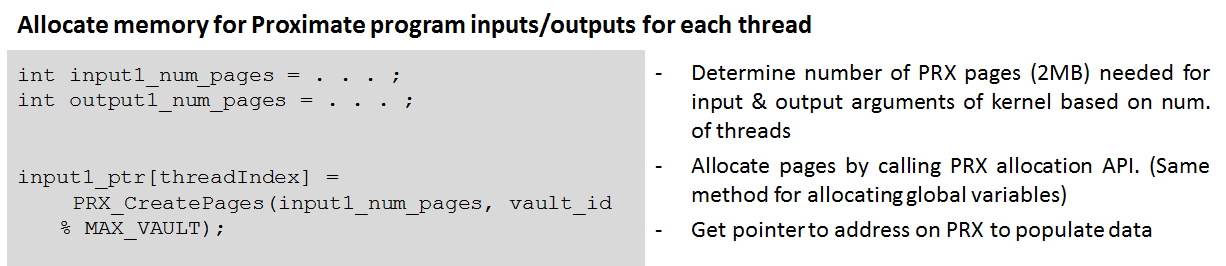
\includegraphics[width=\linewidth]{cs758-figs/api-copy.png}
  \end{center}
\vspace{-0.2in}
  \caption{API for Input Arguments Memory Allocation}
  \label{fig:api-mem}
\vspace{-0.05in}
\end{figure}

\begin{figure}
  \begin{center}
    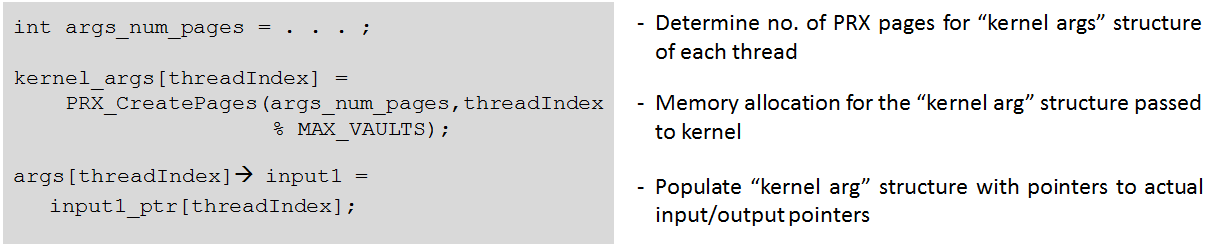
\includegraphics[width=\linewidth]{cs758-figs/api-arg.png}
  \end{center}
\vspace{-0.2in}
  \caption{API for Kernel Argument Structure Allocation}
  \label{fig:api-arg}
\vspace{-0.05in}
\end{figure}

Figure~\ref{fig:api-mem} shows the code snippet for 
memory allocation of input and output arguments required for the computation.
This API can used by the programmer to allocate required number of pages on the Proximate side. 
The input argument is the number of pages required. The size of each page is 1 MB, chosen based on our 
analysis of the per-kernel data set size that are suitable for the target workloads. 
The return value is the virtual address of the next free page in the host mmap’ed heap space. 

Since, \emph{pthread} based kernels only take a single argument, we
need to pack all the input/output arguments into a global structure and pass the address of that
structure to kernel. So, to achieve this Proximate uses the same memory allocation
based \emph{PRX\_CreatePages} API for a global "args" structure.
Figure~\ref{fig:api-arg} also hows how a global "args" structure is created and memory is allocated for the same. 

\paragraph{Kernel Enqueuing and Waiting}

\begin{figure}[h]
  \begin{center}
    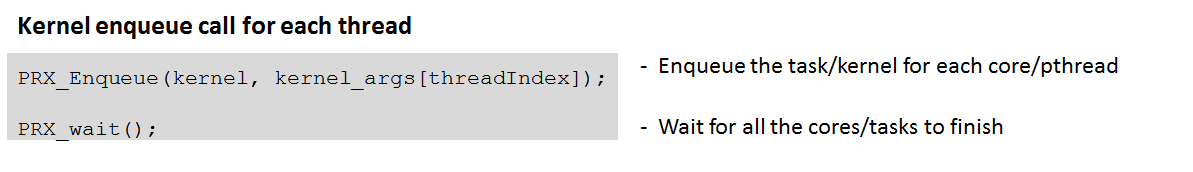
\includegraphics[width=\linewidth,height=1in]{cs758-figs/api-q.png}
  \end{center}
\vspace{-0.2in}
  \caption{API for Kernel Enqueuing and Synchronization}
  \label{fig:api-q}
\vspace{-0.05in}
\end{figure}

This API can be used by the programmer to offload a kernel for computation on the Proximate compute tile. 
The input arguments are: Kernel page index in the Proximate space (return value of \emph{PRX\_LoadKernel} ), and
virtual address (in the host mmap’ed space) of the argument structure which is the only allowed argument to the kernel. 
The argument structure might look like the one shown in Figure~\ref{fig:api-arg}. 
Note that Proximate physical memory space for the argument structure and for each of input array, 
output array and global variable pointers within that structure, must be allocated using \emph{PRX\_CreatePages} before calling \emph{PRX\_Enqueue}.
The programmer also uses \emph{PRX\_Wait} API to wait for all Enqueue’ed kernels to finish execution. There are no input arguments or return value.


\paragraph{Memory Free}

The programmer can use the API shown in Figure~\ref{fig:api-free} to update the memory to indicate that the set of pages associated with this allocation are now free.
\begin{figure}[h]
  \begin{center}
    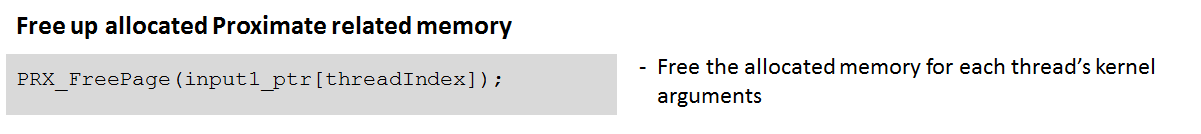
\includegraphics[width=\linewidth]{cs758-figs/api-free.png}
  \end{center}
\vspace{-0.2in}
  \caption{API for Memory Freeing}
  \label{fig:api-free}
\vspace{-0.05in}
\end{figure}

There are some explicit API calls for memory copying to the sharded structures,
but not indicating them here because of the space constraint. One can imagine them
to be very much similar to \emph{CUDA\_MemCpy} based API calls. 


\subsection{Proximate Task Based Queuing Model}\label{sec:queue}

In order to facilitate an efficient task offloading scheme, 
we need a queuing model in order to take in the kernel offload requests 
and schedule them efficiently on the cores or softbrain.
So, we extended the kernel scheduler of proximate to support a simple
queuing model which is based on the MIT Swarm based task model~\cite{jeffrey2016unlocking, jeffreyswarm}.

\begin{figure}[h]
  \begin{center}
    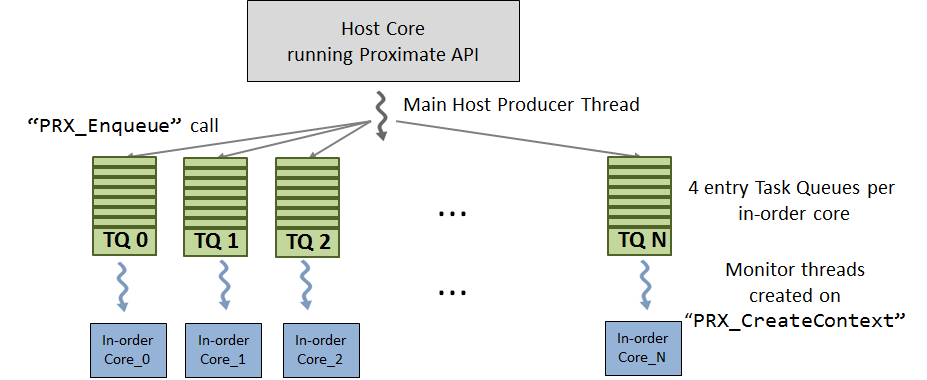
\includegraphics[width=0.9\linewidth, height=2.5in]{cs758-figs/q-model.png}
  \end{center}
\vspace{-0.2in}
  \caption{Proximate Task Based Queuing Model}
  \label{fig:q-model}
\vspace{-0.05in}
\end{figure}

Figure~\ref{fig:q-model} shows the high-level overview of the
Proximate queuing model which is implemented in ZSim simulator.
In this task based model, each in-order core has a 4 entry task-queue (TQ)
able to store the offloaded tasks/kernels. When the runtime on host core
calls the \emph{PRX\_CreateContext} with the number of pthread instances to be launched, 
that manu \emph{monitor threads} are created for each in-order to monitor the per-core
task queue. These monitor threads are always running threads monitoring the task-queue for new work, 
and destroyed only when the \emph{PRX\_Free} API is called.

Everytime, the host core running the proximate runtime offloads a task
using, \emph{PRX\_Enqueue} the task is scheduled on one of the task-queues on a round-robin fashion.
And when the task-queue gets full, the task scheduler will notify the host core not to issue anymore
kernel calls. We do not have a sophisticate load balancer one would need when handling with many kernels, 
but we consider that as a part of future work. 

